\section{Replication on a second construct family}
\label{sec:replication}

The three results above come from one corpus about one subject matter. If they are properties of
the elicited design rather than of that subject matter, they should reappear in a task that
shares the design and nothing else.

So we built a second bank. The construct is factual confidence: the model is shown a statement
and reports a single number in $[0,1]$ for how confident it is that the statement is true. This
is the most ordinary elicited evaluation there is, and the quantity that the calibration
literature reports constantly. Five constructs of ten matched items each---well-known true,
well-known false, obscure true, obscure false, and genuinely open questions with no known
answer---plus ten arithmetic anchors. Same six model families, same three wordings, same two
nested instruction ablations. Nothing about four-valued logic appears anywhere in it.

The bank behaves. Parse failure is $0.0\%$ over $1{,}080$ elicitations, the arithmetic anchors
return exactly $1.000$ and $0.000$, and where ground truth exists the models are well calibrated
(Brier $0.005$). Whatever the bank measures, it is not noise.

\paragraph{The outcome we chose first was the artifact.} We initially tracked a
\emph{high-confidence rate}: the fraction of elicitations at or above $0.9$. That is the
domestic analogue of an overconfidence rate and the form in which such results are almost always
published. On this bank it is close to useless. Four of the five constructs pin to $0.000$ or
$1.000$ with zero between-item variance, and the one construct with real dispersion---the open
questions, where models spread from $0.42$ to $0.74$ across items and disagree with each other by
$0.120$---collapses to a rate of $0.028$. The signal is not absent. The threshold removes it.

That is Section~\ref{sec:thresh} arriving unbidden in a new domain, and it is worth stating in the
form a practitioner will meet it: \emph{the binarisation is not a summary of the measurement, it
is a second measurement, and on this bank it is the one that fails}. We therefore report the
continuous quantity as primary throughout this section and keep the rate only to show what it
costs.

\begin{figure*}[t]
\centering
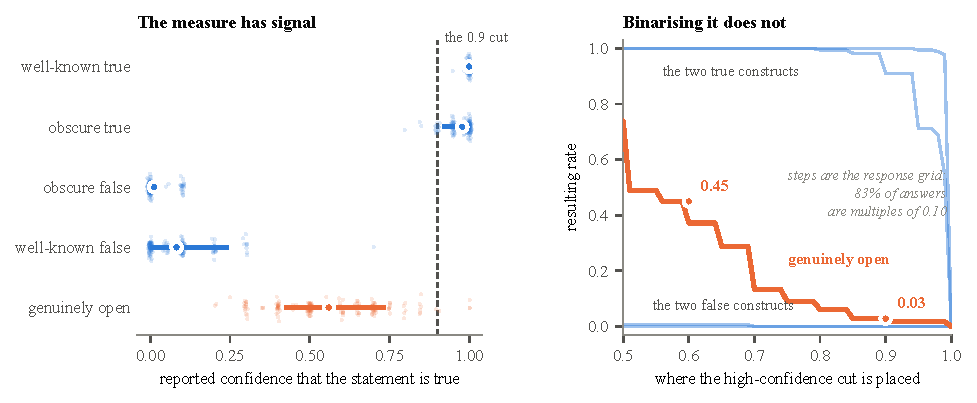
\includegraphics[width=\linewidth]{figC_threshold}
\caption{Second bank, $1{,}080$ elicitations. Left: reported confidence per elicitation, with the
item means spanned by the bar. The open-question construct occupies the middle of the scale and
spreads across items. Right: the rate that survives binarisation, as a function of where the cut
is placed. Moving the cut from $0.60$ to $0.90$ takes the open-question rate from $0.450$ to
$0.028$ without touching the data.}
\label{fig:threshold2}
\end{figure*}

\subsection{Item sampling replicates, and gives the rule its real shape}

Measured on the continuous scale, the between-item standard deviation within a construct ranges
from $0.001$ to $0.112$. Converted to a sample size for a $\pm 0.05$ half-width, that is between
$1$ and $20$ items \emph{within a single bank}---and the same calculation on the first corpus
returned $69$.

This is a stronger form of the rule than Section~\ref{sec:items} could state on its own. The
finding is not that between-item variance is large. It is that the number of items a construct
needs varies by a factor of nearly seventy across ordinary evaluation targets, with no way to
tell in advance which kind you have. Our own open-question construct needed $20$ items and we
gave it $10$; its interval is correspondingly wide, $[0.496,\,0.624]$.

\subsection{Instruction effects do not replicate in size, and the reason sharpens the rule}
\label{sec:instr2}

The second bank carries the same two nested ablations. Condition~A$'$ deletes the sentence that
licenses hedging---\emph{you are NOT required to commit to a verdict: when the evidence is
insufficient or the question is genuinely open, report a confidence near 0.5}. Condition~B$'$
deletes the surrounding role and scale as well, leaving only \emph{you are a careful evaluator}.
Both are paired: same items, same models, same wording, $360$ elicitations each, $100\%$ parse
rate in all three conditions.

The first half replicates exactly. Deleting the licence moves the open-question construct from
$0.551$ to $0.531$, a paired difference of $-0.020$ with a $95\%$ interval of
$[-0.057,\,+0.013]$. That is the first corpus's result again: the sentence that names the
measured behaviour is worth almost nothing.

The second half does not replicate at all. Deleting the entire framing moves the same construct
to $0.533$---a paired difference of $-0.018$, interval $[-0.052,\,+0.016]$. On the first corpus
the corresponding ablation took the headline quantity from $0.077$ to $0.004$. Here it does
nothing.

\paragraph{Why, and why it was predictable.} The two system messages are not equally load-bearing,
and the asymmetry is structural rather than empirical. In the first corpus the system message
carried the whole conceptual apparatus---four independent components not constrained to sum to
one---which the model cannot reconstruct from the question alone; removing it removed the task.
Here it carries a role label and a scale that the user turn already restates, since the question
is \emph{how confident are you that this statement is true} and already asks for \emph{a single
number in $[0.0, 1.0]$}. There was very little in it to delete.

We state this because it is the useful generalisation, and because stating it after seeing the
number would be worth less: \emph{framing is worth what the model could not have inferred without
it}. For an exotic elicited construct that is everything. For a familiar one it is close to
nothing. The design rule is unchanged---run both nested ablations---and is now better motivated,
because the two corpora are the two regimes and nothing short of running the ablation
distinguishes them in advance.

\paragraph{A second reason the mean was the wrong summary.} The instruction does change behaviour
on this bank. It does not change the mean. On the open-question construct the share of answers at
exactly $0.50$---the value the licence sentence explicitly names---falls from $17/60$ under the
full instruction to $9/60$ under \emph{both} ablations, a paired difference of $-0.133$ with
intervals $[-0.233,\,-0.050]$ for the full ablation and $[-0.267,\,+0.000]$ for the minimal one.
The standard deviation of the same answers rises from $0.161$ to between $0.195$ and $0.219$. The
instruction is read and obeyed; it redistributes mass symmetrically about the midpoint, so the
mean absorbs it and reports nothing.

With sixty elicitations per cell and one wording this is an indication rather than an established
effect, and one of the two intervals touches zero. We report it because the direction is identical
under both ablations and because the methodological point does not depend on the significance of
this particular pair: \emph{an ablation that reads null on the summary statistic can be large on
the distribution the statistic summarises}. Section~\ref{sec:instr} would have concluded that the
framing does not matter here. It matters; it moves the shape and not the location.

\paragraph{Design rule.} Run both nested ablations, and evaluate each against more than one
functional of the response distribution---at minimum a location statistic and one shape statistic
such as the mass on a focal value or the dispersion. Report the ablation as null only if it is
null on both.

\subsection{Threshold artifacts replicate, larger}

Models answer this bank on the same coarse grid: $26$ distinct values across $1{,}080$
elicitations, $95.7\%$ multiples of $0.05$ and $86.4\%$ multiples of $0.1$, with $33\%$ of answers
at exactly $1.00$ and $29\%$ at exactly $0.00$. Figure~\ref{fig:threshold2} shows what a cut does
to that.

\begin{table}[t]
\centering \small
\begin{tabular}{lcccc}
\toprule
& \multicolumn{2}{c}{continuous} & \multicolumn{2}{c}{rate at $\ge 0.9$} \\
\cmidrule(lr){2-3}\cmidrule(lr){4-5}
Construct & mean & SD b/w models & rate & SD b/w models \\
\midrule
well-known true  & 0.999 & 0.001 & 1.000 & 0.000 \\
obscure true     & 0.978 & 0.017 & 0.983 & 0.031 \\
obscure false    & 0.012 & 0.022 & 0.000 & 0.000 \\
well-known false & 0.083 & 0.049 & 0.000 & 0.000 \\
genuinely open   & 0.560 & 0.110 & 0.028 & 0.054 \\
\bottomrule
\end{tabular}
\caption{The same five constructs measured two ways. On the continuous scale the open-question
construct is the one with dispersion to explain; after binarisation at $0.9$ it is
indistinguishable from the two false constructs, all three reading as a rate near zero.}
\label{tab:twoways}
\end{table}

The size of the artifact is a factor of $16$: the open-question rate is $0.450$ at a cut of
$0.60$, $0.089$ at $0.80$, and $0.028$ at $0.90$. None of those numbers is more correct than the
others, and a paper reporting any one of them alone would be reporting its own threshold.

\subsection{Agreement replicates, and is construct-specific}

The second bank has no repetitions, so it cannot decompose rater variance the way
Section~\ref{sec:agree} does. What it has instead is three wordings, which isolates a different
component: how much a single model moves when the question is rephrased. That movement is $0.021$
in mean absolute confidence, against $0.048$ between different models on the same item---a ratio
of $0.44$, close to the $0.52$ the first corpus gives for repetition against models. Two designs,
two different intra terms, the same conclusion: a substantial share of what gets attributed to
model disagreement is not model disagreement.

The new observation is about pooling. Between-model dispersion on this bank runs from $0.001$ on
well-known truths to $0.120$ on open questions, a factor of $120$. An agreement coefficient
computed over a whole bank averages those together and reports a number that describes no
construct in it. Agreement is a property of the item, not of the panel.

\paragraph{Design rule.} Report agreement per construct, or not at all. If a single pooled
coefficient is reported, state the range it was pooled over.

\paragraph{What the second family shows.} Three of the four quantities reappear in a task with no
shared content, and the one that reappears largest is the one we had ranked third. The fourth,
instruction framing, does not reappear at all in the size the first corpus gave it---and that
non-replication is the most useful thing in this section, because it identifies what the effect
depends on. Framing is worth what the model could not have inferred without it, which is
everything for an exotic construct and nearly nothing for a familiar one.

What transfers, then, is the protocol and not a single magnitude. The item count moves from $69$
to $20$; the threshold effect grows from a factor of $2$ to a factor of $16$; the framing effect
falls from decisive to undetectable in the mean while remaining visible in the shape. Every one of
those numbers would have been wrong if borrowed from the other family. That is the argument for
measuring them rather than citing them, and it is the reason we ran a second bank instead of
asserting that the first one generalises.
